\documentclass[11pt]{article}

\usepackage[style=numeric, natbib]{biblatex}
\usepackage[margin=20ex]{geometry}
\usepackage{amsmath}
\usepackage{array}
\usepackage{booktabs}
\usepackage{caption}
\usepackage{fancyvrb}
\usepackage{graphicx}
\usepackage{hypdoc}
\usepackage{libertine}
\usepackage{longtable}
\usepackage{newtxmath}
\usepackage{tabularx}
\usepackage{zi4}
\usepackage{graphicx}
\usepackage{colortbl}
\usepackage{microtype}
\usepackage{balance}
\usepackage{mathtools}
\usepackage{float}
\usepackage{color}
\usepackage{listings,lstlangcoq}
\usepackage[dvipsnames]{xcolor}
\usepackage[all]{xy}
\usepackage{xspace}

\lstdefinestyle{customcoq}{
  columns=flexible,
  mathescape=true,
  belowcaptionskip=1\baselineskip,
  breaklines=true,
  xleftmargin=\parindent,
  language=Coq,
  morekeywords={Variant, fun, Arguments, Type, cofix},
  % morekeywords={SOCKAPI,ITREE,data_at,data_at_},
  emph={%
    SOCKAPI,ITree,data_at,data_at_
  },
  emphstyle={\bfseries\color{green!40!red!80}},
  showstringspaces=false,
  basicstyle=\small\ttfamily,
  keywordstyle=\bfseries\color{green!20!black},
  commentstyle=\itshape\color{red!40!black},
  identifierstyle=\color{violet!50!black},
  stringstyle=\color{orange},
  escapeinside={<@}{@>}
}
\newcommand{\inlinecoq}[1]{\mbox{\lstinline[style=customcoq,columns=fixed,basewidth=.48em]{#1}}}
\newcommand{\ilc}[1]{\inlinecoq{#1}}

\addbibresource{references.bib}

\newcommand{\leon}[1]{\textcolor{blue}{#1}}
\newcommand{\gr}[1]{\textcolor{Orange}{#1}}
\newcommand{\yz}[1]{\textcolor{ForestGreen}{#1}}
\newcommand{\yzt}[1]{\textcolor{ForestGreen!50}{#1}}
\newcommand{\cut}[1]{\textcolor{Gray!40}{#1}}

\newtheorem{theorem}{Theorem}
\newtheorem{definition}{Definition}
\newtheorem{example}{Example}

\newcommand{\ocfg}{OCFG\xspace}
\newcommand{\pat}{\texttt{Pat}\xspace}

\hypersetup{colorlinks=true, linkcolor=black}

\begin{document}

\title{CFG Patterns: A new tool to formally verify optimisations in Vellvm}

\author{Leon Frenot\\ Supervised by Yannick Zakowski \& Gabriel Radanne}

\date{February 5th, 2024 - July 5th, 2024}

\begin{titlepage}
  \centering
  {\textsc{École normale supérieure de Lyon} \par}
  \vspace{1cm}
  {\Large \textsc{Internship Report}\par}
  \vspace{1.5cm}
  {\huge\bfseries CFG Patterns: A new tool to formally verify optimisations in Vellvm\par}
  \vspace{2cm}
  {\Large\itshape Leon Frenot\par}
  \vfill
  supervised by\par
  Yannick~Zakowski~\&~Gabriel~Radanne\par
  at ENS Lyon
  \vfill

  % Bottom of the page
  {\large February 5th, 2024 - July 5th, 2024\par}
\end{titlepage}

\tableofcontents
\newpage

\hypersetup{colorlinks=true, linkcolor=red}

% \begin{abstract}
%   \leon{Abstract}
% \end{abstract}

\section{Introduction}
\label{sec:intro}

\indent
For my M2 year at ENS de Lyon, I completed a 20 weeks internship in the LIP Computer Science laboratory in ENS Lyon. This internship was supervised by Yannick Zakowski and Gabriel Radanne in the Compilation and Analysis, Software and Hardware Team of the LIP. The goal of this internship was to design and implement a pattern language over control flow graphs to provide a framework for formal proofs on optimizations.

\paragraph{}
Compilers are extremely complex objects, gcc's source code is made of about 15 million lines of code~\cite{GCC}. Because of that complexity, it can be hard to assert that compilers follow their specification. For instance, code compiled for aeronautics is usually done without optimizations to reduce the likelihood of unintended behaviors.

One possible solution to this dilemma is \emph{verified compilation}. That is, compilers that are proven to preserve the semantics of the source code. Proving this implies defining formal definitions for the semantics of the source language, the target language and proving the preservation of behavior between them. Verified compilers usually rely on proof assistants like Coq~\footnote{\url{https://coq.inria.fr/}}, which allow writing executable code, i.e.\ the compiler, and formal proofs on that code.

Verified compilers have been a research subject for some time now, notably since the CompCert project~\cite{CompCert}, which established a verified compiler for the ISO C 99 language. It is commercialized by AbsInt~\footnote{\url{https://www.absint.com/}}, for industries like nuclear and aeronautics. Our work takes place in the context of the Vellvm project~\cite{Vellvm}, which aims at formalizing the semantics of LLVM IR\@. LLVM IR is an intermediate representation used as a front-end and back-end for many languages and architectures. It is based on a Control-Flow Graph (CFG) model, with named blocs and abstract registers.

Vellvm has had some applications, notably to prove some IR to IR optimizations~\cite{Vellvm}, as well as to establish a verified front-end from Helix to LLVM IR~\cite{Helix}. One key challenge that was identified from establishing that front-end was fresh identifier generation. This is a reoccurring issue with formal proofs on named systems~\cite{Bastien}. This observation calls for better abstraction for reasoning on graphs. Previous experiments aimed at designing combinators to ease the construction of graphs capturing high-level control flow abstractions, a solution suitable to write front-ends.

\paragraph{}
My work focused on a orthogonal notion. When writing optimization passes, there is often a need to identify a subgraph with specific structural properties, apply a transformation on it, and link the transformed subgraph back with the context.

To address this problematic, I designed a \emph{Domain Specific Language} (DSL) of \emph{patterns} over graphs, \pat{}. It is equipped with a \emph{matcher} which, given a graph, computes the set of \emph{decompositions} that match a given pattern. This matcher is proven to follow a specification capturing at a higher level the structural properties expressed by \pat{}.

Following this, I wrote an implementation of the Block Fusion optimization based on \pat{}, and proved it preserves the semantics of the graph. To establish this proof, I have on the one hand proved a generic substitution theorem, and on the other hand leveraged the specification of a pattern to show the structural properties of a captured subgraph matches the requirements for the optimization.

In the remaining of this report, Section~\ref{sec:background} introduces the necessary prerequisites on Interaction Trees and Vellvm. Section~\ref{sec:lang} describes the \pat{} DSL and its semantics. And finally, Section~\ref{sec:deno} covers the Block Fusion case study.

\section{Background}
\label{sec:background}

\subsection{LLVM and Vellvm}

\leon{TODO: figures (vir syntax and intrep stack)}

The goal of the Vellvm project is to \emph{formally define} the semantic of the LLVM IR and build verified
components based on that formalization.
%
LLVM~\cite{LLVM} is a compiler infrastructure designed around a language-independent \emph{intermediate representation} (IR). It is used to develop frontends for programming languages and backends for instruction set architectures.

The LLVM IR is an instruction set similar to low-level assembly languages like RISC, but features high-level informations. This duality allows it to represent any program while still permitting analysis and optimizations. It is based on control flow-graphs, with named labels and registers, and guarantees Single Static Assignment (SSA) form, which is key to many static analyses and optimizations. The LLVM IR is statically typed, and features integer-pointer casts.
%
Optimizations and analysis on the LLVM IR are done through successive \emph{analysis and transformation passes}.

\subsection{Interaction Trees}

The core of Vellvm's formalization relies on Interaction Trees~\cite{ITrees} (ITrees).

ITrees are a data structure designed to represent the dynamic behaviors of a computation. Itrees are a coinductive structure, meaning they represent potentially infinite trees. This allows ITrees to model recursive and effectful programs, including divergent computations.

Figure~\ref{fig:itree} show the Coq definition of ITrees. It has two parameters: an \emph{event} type \ilc{E: Type -> Type}, and a \emph{return} type \ilc{R: Type}. The definition uses three constructors: \ilc{Ret} corresponds to halting and returning a value of type \ilc{R}; \ilc{Tau} corresponds to a \emph{silent step}, i.e. an internal computation, followed by computation \ilc{t}; and \ilc{Vis} corresponds to a \emph{visible event}, it describes an external computation \ilc{e} which returns a value of type \ilc{A}, and a continuation \ilc{k} which depends on that return value.

\begin{figure}
  \begin{lstlisting}[style=customcoq,basicstyle=\small\ttfamily]
CoInductive itree (E : Type -> Type) (R : Type) : Type :=
  | Ret (r : R)
  | Tau (t : itree E R)
  | Vis {A : Type} (e : E A) (k : A -> itree E R).
  \end{lstlisting}
  \caption{The \ilc{itree} datatype}
  \label{fig:itree}
\end{figure}

\citet{ITrees} provide concrete examples of ITrees. For example, we can define an effect type \ilc{IO}, corresponding to simple inputs and outputs over integers. With \ilc{IO}, we can establish an ITree \ilc{echo} which loops forever, echoing each input received to the output:
\begin{lstlisting}[style=customcoq,basicstyle=\small\ttfamily]
Inductive IO : Type -> Type :=
  | Input : IO nat
  | Output : nat -> IO unit.

CoFixpoint echo : itree IO void :=
  Vis Input (fun x => Vis (Output x) (fun _ => echo)).
\end{lstlisting}

Effects can easily be added or removed from the semantics of an ITree. The \ilc{Vis} constructor represents \emph{uninterpreted events}. By defining an \emph{event handler}, semantics are assigned to these events. Interpreting an ITree then consists of folding that handler over the ITree. This allows the semantics of ITrees to be \emph{modular}.
Furthermore, the semantics of ITrees are also \emph{compositional} with the use of \emph{combinators}. For example, composing ITrees can be handled by the combinator \ilc{bind}.

To reason over ITrees, we have multiple notions of \emph{bisimilarity}. The most relevant one for our work is \emph{weak bisimilarity}, noted \ilc{t1 ≈ t2}. We say that \ilc{t1 ≈ t2} if they return the same value, and have the same visible events. Notably, this relation is an equivalence ``up-to-Tau'', in the sense that we have \ilc{Tau t ≈ t} and \ilc{t ≈ Tau t}. 
% This equivalence can be refined up to a relationship $R : A \rightarrow B \rightarrow Prop$: we then have $\ilc{Ret}\; a \approx_R \ilc{Ret}\; b \iff R\; a\; b$.
% \gr{Tout sert la dedans ? Je pense qu'il ne faut présenter que ce dont tu vas avoir besoin. Aussi: cite}

Unlike similar projects, which rely on \emph{operational semantics} and simulation diagrams, ITrees rely on \emph{denotational semantics}. It is based on equations that can be used to prove bisimulation. These equations allow the user to reason without using coinductive reasoning or the definition of the weak bisimulation. The compositionality of the semantics also allow simpler reasoning than operational semantics, since program counter and similar notions are lifted away.

\subsection{Vellvm's semantics}

Vellvm introduces Verified LLVM IR (VIR), a \emph{realistic subset} of the LLVM IR.
% Figure~\ref{vir} shows a subset of VIR's syntax.

Each element of VIR's syntax is represented by a corresponding ITree. Each effect (except control flow) is captured by a \ilc{Vis} event, which can be interpreted later. This semantic includes many non-trivial features of LLVM IR, including pointers, LLVM's $\phi$-nodes and undefined behaviors.

Since the semantics of a block or set of blocks can be defined without relying on a ``complete'' CFG, it is possible to use ``open control-flow graphs'' (\ocfg), which is simply a set of blocks without a defined entry point.

To interpret the semantics of the different effects of its syntax, Vellvm uses a stack of interpreters. It gradually introduces external elements to the semantic (intrinsics, global and local environments, \ldots). Figure~\ref{fig:interp} show that stack of interpretation. The final levels split between a \emph{propositional} model, which interprets the non-determinism of LLVM IR's undefined behaviors, and an \emph{executable} model, which implements one of these behaviors.

Since this internship mainly focused on structural properties, we will only interact with level 0. That is, with control flow as the only interpreted events.

\begin{figure}
  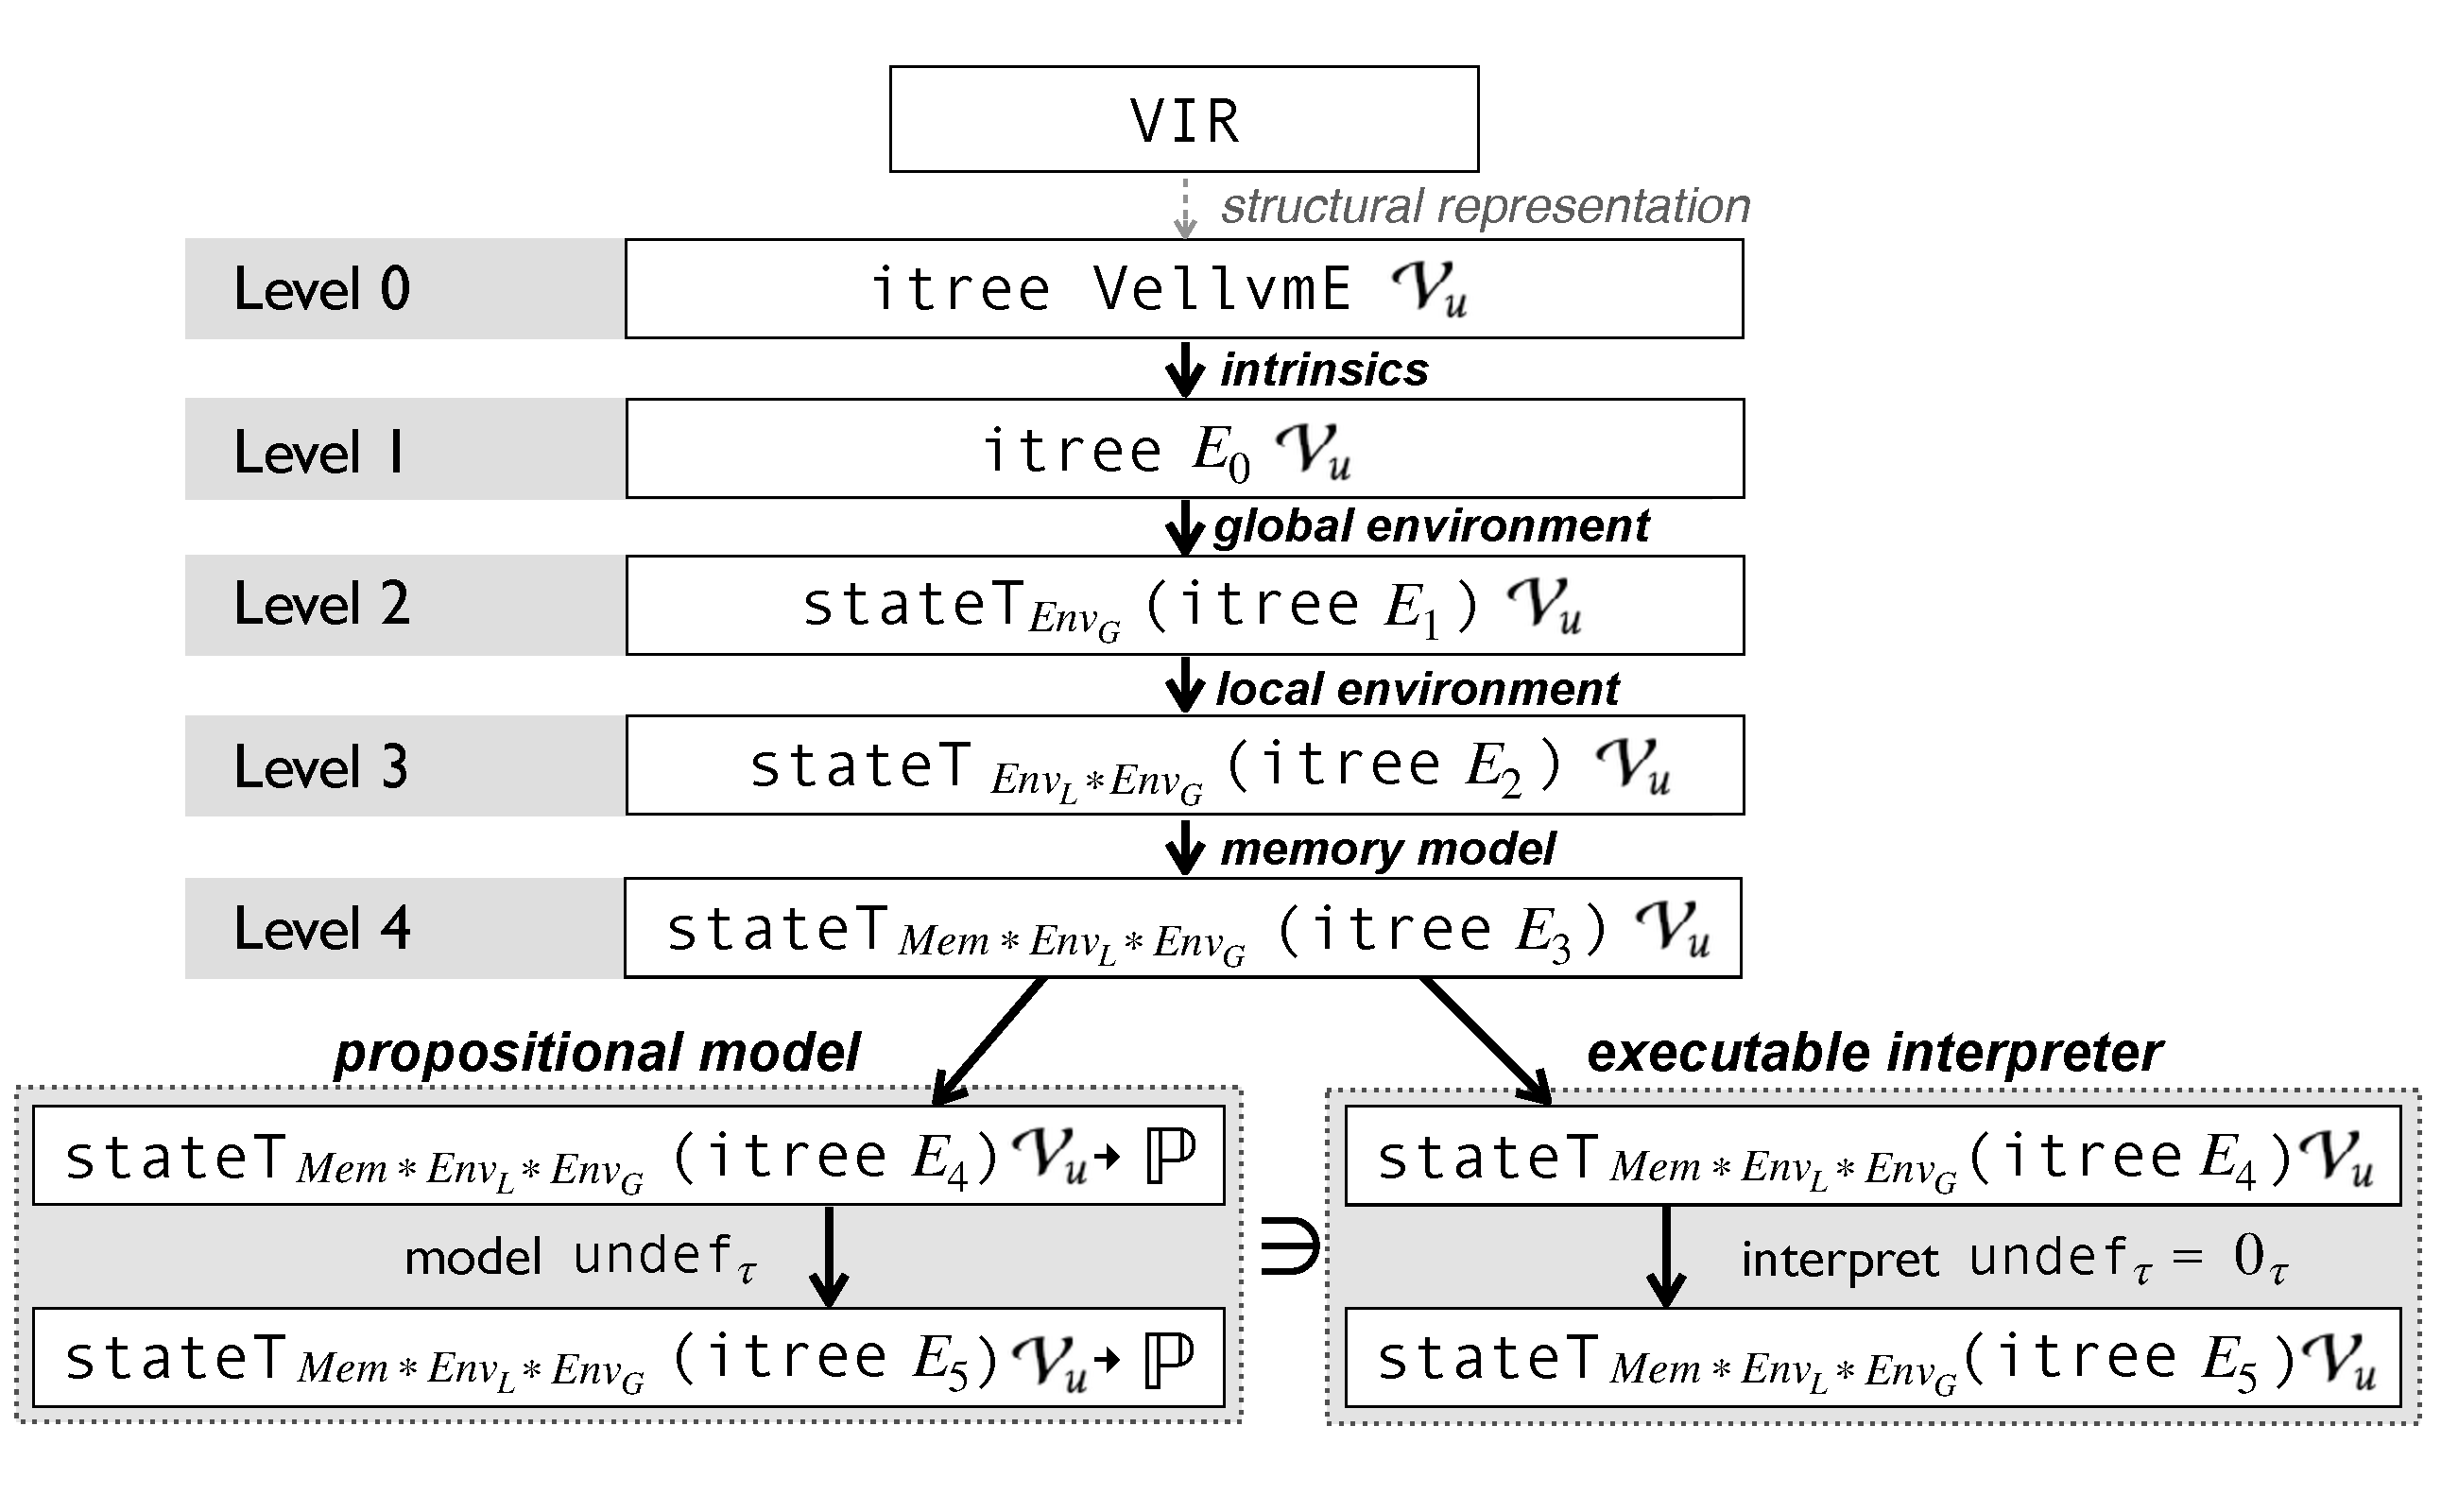
\includegraphics[width=\textwidth]{images/interp-figure.pdf}
  \caption{Vellvm's levels of interpretation}
  \label{fig:interp}
\end{figure}

\section{The pattern language}
\label{sec:lang}

% \yz{De façon générale, commencer par des bullet points ou des séries de paragraphe est excellent, mais c'est important de lui donner corps en rédigeant dans un second temps un texte cohésif. Je tente une proposition rapide par exemple pour ce chapeau pour illustrer.}

% \yz{Remarque générale : il faut utiliser beaucoup beaucoup de macros quand on écrit du TeX. Par exemple OCFG va apparaître beaucoup, et on peut hésiter sur la façon de le typeset/écrire : macro }

% \yz{Il peut être pratique d'avoir un nom pour ton langage pour pouvoir y référer.}

\yzt{We now turn our attention to the central piece of our contribution: the design of \pat{}, a DSL of patterns for writing and proving correct program transformations. This DSL is composed of two core components. First, an indexed datatype provides a syntax for the user to specify how they wish to decompose an input \ocfg. Second, a \emph{matcher} provides a semantics to the language, specifying the valid decompositions associated to each pattern. Finally, we illustrate on an example the definition and semantic characterization of a pattern extracting the heads of a graph, written in our DSL.}

In this section we will focus on our main contribution: the design of \pat{}, a DSL of patterns for writing and proving correct program transformations. This DSL is composed of two core components. The first is a datatype, \ilc{Pattern}, which provides a syntax for the user to specify how they wish to decompose an input \ocfg. The second is a \emph{matcher} function, which provides semantics to apply the language to an \ocfg{}, specifying the valid decompositions associated to each pattern. Finally, we illustrate on an example the definition and semantic characterization of a pattern extracting the heads of a graph, written in our DSL\@.

% \cut{
% In this section we will:\begin{itemize}
%   \item Define a Domain Specific Language that can capture optimizable subgraphs in an \ocfg\@.
%   \item Introduce a matcher on this language and the corresponding semantics of each constructor.
%   \item Present the Coq implementation of the language, matcher and semantics.
% \end{itemize}
% }

\subsection{\pat: a DSL for pattern matching on graphs}

\yzt{At a high level, we look for a language allowing the user to characterize and reason about optimizable subgraphs in an \ocfg. 
To this end, we introduce \pat, a general, very expressive DSL for pattern matching on graphs. The specific patterns we are interested in from the perspective of compilation will then be expressed in \pat.}

\begin{figure}
  \begin{lstlisting}[style=customcoq,basicstyle=\small\ttfamily]
    Inductive Pattern : Type -> Type :=
    | Graph: Pattern ocfg
    | When: forall  {S}, Pattern S -> (S -> bool) -> Pattern S
    | Map: forall  {S} {T}, Pattern S -> (S -> T) -> Pattern T
    | Focus: forall  {S}, Pattern S -> Pattern (ocfg * S)
    | Block: forall  {S}, Pattern S -> Pattern (block_id * blk * S)
    | Head: forall  {S}, Pattern S -> Pattern (block_id * blk * S)
    | Branch: forall  {S}, Pattern S -> Pattern (block_id * blk * S)
  \end{lstlisting}
  \caption{The \ilc{Pattern} datatype}
  \label{fig:pat}
\end{figure}

Figure~\ref{fig:pat} introduces \pat{}'s syntax, defined as an inductive datatype \ilc{Pattern}.
Because the purpose of a pattern is to decompose a graph into a certain structure, the \ilc{Pattern} datatype reflects this intention by taking as argument a type, which represents the return type of the pattern.\footnote{Such families of types are common in dependently typed languages, and are referred to as Generalized Algebraic Data Types in languages such as OCaml or Haskell.}
This typing information is leveraged in the definition of the matcher, introduced in Section~\ref{sec:matcher}: matching a pattern of type \ilc{Pattern S} will always return elements of type \ilc{S}.

The \ilc{Pattern} type is build of seven constructors. The only base case is the \ilc{Graph} constructor which trivially match any graph and does not perform any decomposition. On more traditional paper presentation, it corresponds to a single hole $\square$.

The six other constructors recursively decompose the graph, typically enriching the return type of the pattern in doing so. 
The \ilc{When} constructor acts as a filter:
given a pattern of return type \ilc{S}, it builds a pattern with the same return type, but takes as argument a filtering function \ilc{S -> bool} used to restrict the set of matching graphs to those satisfying the condition.
The \ilc{Map} constructor simply hardcodes functoriality into the datatype, allowing for post-processing the output of a pattern by a pure function. That is: given a return type \ilc{S} and a function \ilc{S -> T}, it builds a pattern of return type \ilc{T}.
The \ilc{Focus} constructor, given a pattern \ilc{P}, builds a pattern that tries to match \ilc{P} on any subset of the graph given as argument.
The \ilc{Block} constructor extracts any block from the graph and matches the pattern given as argument against the rest of the graph.
The \ilc{Head} constructor extracts a block without predecessors from the graph and matches the pattern given as argument against the rest of the graph.
The \ilc{Branch} constructor extracts a block whose terminator is a branch from the graph and matches the pattern given as argument against the rest of the graph.

\paragraph*{An example of pattern: block fusion.}
We illustrate the use of \pat{} to implement\footnote{Or rather, to \emph{specify} such an optimization. We discuss briefly executability in conclusion.} a bloc fusion optimization.
Block Fusion typically consists of finding two blocks (A and B) such that A is the only predecessors of B, B is the only successor of A, and B is not the graph's entry point. Since an execution of A is always followed by B, and an execution of B is always preceded by A, we can replace them by a single block that follows the execution of both A and B.

The applicable subgraphs are specified with the pattern:
\begin{lstlisting}[style=customcoq,basicstyle=\small\ttfamily]
pfusion := When (Block (Head Graph)) BlockFusion\_f
\end{lstlisting}
The pattern starts with \ilc{Block} to match any block \ilc{A} Then, \ilc{Head} matches a block \ilc{B} that has no predecessors (except possibly \ilc{A} as it is not in scope of the pattern anymore), and finally \ilc{When _ BlockFusion\_f} asserts that \ilc{B} is the only successor of \ilc{A}.

\begin{figure}
  \xymatrix{
    &&&&\\
    &*+[F]\txt{\ilc{A}\\\ilc{Block}: any block}\ar[dd]&&\;\ar@{-->}`u[ul] `[ll] [ll]&\\
    *+[F.]\txt{\ilc{When _ BlockFusion_f}\\ asserts that \ilc{B} is\\the only successor of \ilc{A}}\ar@{..>} [r]&&&\txt{Graph}\\
    &*+[F]\txt{\ilc{B}\\\ilc{Head}: no predecessors\\once \ilc{A} is removed}\ar@{-->}`d[dr] `[rr] [rr]&&&\\ 
    &&&
    \save "2,3"."4,5"*[F--]\frm{} \restore
  }
  \caption{The \ilc{pfusion} pattern}
  \label{fig:gfusion}
\end{figure}

Figure~\ref{fig:gfusion} illustrates graphically the shape of the graph decompositions that match \ilc{pfusion}. The full lines (\ilc{A, B} and the arrow between them) represent the parts fixed by \ilc{pfusion}. The dashed lines refer to parts that are allowed, but not necessarily them: other blocks in the graphs with arrows coming towards \ilc{A} or from \ilc{B} (but not in the middle of them). The dotted lines 
show the \ilc{When} constructor.

\paragraph*{Discussion around the constructors}
The set of constructors for \pat is not minimal. Indeed, \ilc{fun p => Block p} could be written as \ilc{fun p => When (Focus p) (fun '(l, _) => size l = 1)}, and \ilc{fun p => Branch p} could be written as\\\ilc{fun p => When (Block p) (fun '(id, b, _) => term_is_branch b)}. Finding a minimal set was not a goal of the DSL as the main concern was ease of use, both for the user, for designing a matcher, and for establishing the meta-theory. 

\ilc{Map} and the functoriality it brings feel natural to add and are easy to implement and prove. But we have no immediate use for it at this time. An argument against \ilc{Map} could be made, as every other constructor allows working backwards to rebuild the graph by recombining the extracted part (as long as it matches with something).

\ilc{Map} also makes \ilc{Head} a minimal constructor. Indeed, while \ilc{Head Graph} can be written as \ilc{When (Block Graph) (fun '(id, b, g) => is_head id g)}, there is no function f such that\\\ilc{Head Map Graph (fun _ => ())} can be written as \ilc{When (Block Map (fun _ => ())) f}, since we loose the information on the rest of the graph.

While a user will want to work using closed instances of pattern, that is objects of type \ilc{Pattern S}, our proofs work on open instances of pattern, that is objects of type\\\ilc{Pattern S -> Pattern (f S)}, to allow compositionality. We will call these objects \emph{opened patterns}. Note that constructors other than \ilc{Graph} are opened patterns.

\subsection{Matcher functions}
\label{sec:matcher}

We now turn to the question of defining the semantics of our patterns, via a \emph{matcher function}. 
A matcher function takes a pattern \ilc{p} and an \ocfg{} \ilc{G} as arguments, and returns a set of decompositions of \ilc{G} that match \ilc{p}.
We have mainly focused on \emph{specifying} patterns, by implementing a matcher that returns \emph{all} valid decompositions. 
Although rather meant as a specification than as a realistic implementation, the \ilc{MatchAll} function, depicted in Figure~\ref{fig:matchall}, is nonetheless executable. This not only allows testing, but also drastically reduces the distance left to bridge to have an efficient implementation that is provably sound.

% \gr{Cette description est le moment crucial, il faut que ca soit beaucoup plus
%   clair ce qu'il se passe}
% \gr{In practice, our matcher turns a list:}
% it computes recursively the decomposition according to the sub-pattern, and flat maps (Definition provided on Figure~\ref{fig:flatmap})\gr{Dit ce que ca fait} a function for each constructor extending the decomposition according to the head constructor.

\ilc{MatchAll} returns a list of each decomposition that matches the pattern. It recursively computes the decomposition according to the sub-pattern. We can identify three way the constructors are computed: \ilc{MatchAll Graph} returns the singleton containing the graph. \ilc{MatchAll When/Map} first computes the sub-pattern and then applies the filter/map function over the resulting list. For the extracting constructors, \ilc{Focus, Block, Head} and \ilc{Branch}, the goal is to first extract an element from the graph, and then apply the sub-pattern.

To extract an element, \ilc{MatchAll} relies on decomposition functions, whose definitions are given in Figure~\ref{fig:match_sub_funs}. These functions each rely on an auxiliary function which is folded over the graph to find each matching element. For example, the \ilc{Focus} constructor relies on the \ilc{focus} function. It folds an auxiliary function \ilc{focus_aux} over the graph to get each subgraph, and then maps an additional function to get the complementary subgraphs. The folding recursively computes each subgraph: it starts with the singleton containing the empty map, and, on each iteration, \ilc{focus_aux} returns a list containing each of the map given as argument, and each of them with a new block inserted.

Extracting an element returns a list of type \ilc{list S*ocfg}. We then have to apply the sub-pattern over the \ocfg on the right hand side. To do that, for each element of the return list, the function \ilc{flat_map_r} (Definition provided on Figure~\ref{fig:flatmap}) matches the sub-patterns to the right-hand side, which gives another \ilc{list T*ocfg}, maps the original left-hand side back on it, so we have a \ilc{list S*T*ocfg}, and appends the resulting lists together. 

\begin{figure}
  \label{fig:match}
  \begin{lstlisting}[style=customcoq,basicstyle=\small\ttfamily]
Fixpoint MatchAll {S} (P: Pattern S) (g: ocfg) : list S :=
  match P with
    | Graph => [g]
    | When p f => filter (fun x => f x = true) (MatchAll p g) 
    | Map p f => map f (MatchAll p g)
    | Focus p => flat_map_r (MatchAll p) (focus g)
    | Block p => flat_map_r (MatchAll p) (blocks g)
    | Head p => flat_map_r (MatchAll p) (heads g)
    | Branch p => flat_map_r (MatchAll p) (branches g)
  end.
  \end{lstlisting}
  \caption{The \ilc{MatchAll} function}
  \label{fig:matchall}
\end{figure}

\begin{figure}
  \begin{lstlisting}[style=customcoq,basicstyle=\small\ttfamily]
Definition flat_map_r {A B C} (f : B -> list C) (l : list (A*B)) : list (A*C) :=
  match l with
    | [] => []
    | (a, b)::q => (map (fun c => (a, c)) (f b))++flat_map_r f q
  end.
  \end{lstlisting}
  \caption{The \ilc{flat_map_r} function}
  \label{fig:flatmap}
\end{figure}
\begin{figure}
  \begin{lstlisting}[style=customcoq,basicstyle=\small\ttfamily]
Definition focus_aux id b acc : list ocfg := acc ++ (map (insert id b) acc).
Definition focus (G: ocfg) := map (fun G' => (G', G ∖ G')) (map_fold focus_aux [∅] G).
  \end{lstlisting}
  
  \begin{lstlisting}[style=customcoq,basicstyle=\small\ttfamily]
Definition blocks_aux (G: ocfg) : (block_id*blk) -> (block_id*blk*ocfg) :=
  fun '(id, b) => (id, b, delete id G).
Definition blocks (G: ocfg): list (block_id*blk*ocfg) :=
  map (blocks_aux G) (map_to_list G).
  \end{lstlisting}
  
  \begin{lstlisting}[style=customcoq,basicstyle=\small\ttfamily]
Definition heads_aux (G: ocfg) id b acc : list (block_id*blk*ocfg) :=
  if is_empty (predecessors id G)
  then (id, b, delete id G)::acc
  else acc.
Definition heads (G: ocfg): list (block_id*blk*ocfg) := map_fold (heads_aux G) [] G.
  \end{lstlisting}
  
  \begin{lstlisting}[style=customcoq,basicstyle=\small\ttfamily]
Definition branches_aux (G: ocfg) id b acc : list (block_id*blk*ocfg) :=
  match b.(blk_term) with
    | TERM_Br _ l r => (id, b, (delete id G))::acc
    | _ => acc
  end.
Definition branches (G: ocfg): list (block_id*blk*ocfg) := map_fold (branches_aux G) [] G.
  \end{lstlisting}
  \caption{\ilc{MatchAll}'s subfunctions}
  \label{fig:match_sub_funs}
\end{figure}

\subsection{Specification}

\yzt{We have claimed that \ilc{MatchAll} \emph{returns all valid decompositions}. We capture this statement by providing specifications for each constructor of \pat, and proving they are exactly captures by \ilc{MatchAll}.}
\gr{For this purpose, we will give a generic specification for \emph{opened patterns}, i.e. patterns parameterized by a sub-pattern.}

A specification for an opened pattern \ilc{PatF} of type \ilc{Pattern S -> Pattern (f S)} is a function \ilc{R_PatF} of type \ilc{ocfg -> Pattern S -> f S -> Prop}. We say that \ilc{MatchAll} is correct for that specification if we have:
\begin{lstlisting}[style=customcoq,basicstyle=\small\ttfamily]
forall (G: ocfg) (pat: Pattern S) (X:f S), X ∈ MatchAll (PatF pat) G IFF R_PatF G pat X
\end{lstlisting}

Similarly, a specification for a closed pattern \ilc{pat: Pattern S} is \ilc{R_pat: ocfg -> S -> Prop}. \ilc{MatchAll} is correct for it if: \ilc{forall (G:ocfg) (X:S), X ∈ MatchAll pat G IFF R_pat G X}. 

\gr{Let us start with} the correction for \ilc{Graph}: \ilc{forall G G', G' ∈ (MatchAll Graph G) IFF G' = G.} Its proof is immediate by definition of \ilc{MatchAll Graph}.

The correction for \ilc{fun P f -> When P f} is given by the following theorem:
\begin{lstlisting}[style=customcoq,basicstyle=\small\ttfamily]
  forall (P: Pattern S) f X G, X ∈ (MatchAll (When P f) G) IFF f X = true \/ X ∈ (MatchAll P G).
\end{lstlisting}
We can also give a theorem for the correctness of \ilc{Map}. Proving their correctness is then immediate using builtin lemmas on \ilc{filter} and \ilc{map}.

The same proof mechanism is used for \ilc{Focus}, \ilc{Block}, \ilc{Head} and \ilc{Branch}. We will now detail it for \ilc{Head}.
%
% \ilc{MatchAll} relies on the \ilc{heads} function to match the \ilc{Head} constructor. The goal of that function is to find all the "heads", i.e. blocks without predecessors, in an OCFG. To do that, it folds a \ilc{heads_aux} function over the map. That function calls the \ilc{predecessors} function on each block, and appends the result to the return list if the block doesn't have predecessors.
%
Figure~\ref{fig:sem_head_def} gives a semantic definition for \ilc{Head}. It is composed of two parts: \ilc{heads_aux_sem} which gives semantics for the auxiliary function, which is used to prove its correctness, and \ilc{heads_sem} which gives the actual semantics for \ilc{Head} and is used to enunciate the \ilc{Pattern_Head_correct} theorem.
%
Finally, as show in Figure~\ref{fig:head_cor} we can prove the semantics for the auxiliary function, the \ilc{heads} function and \ilc{MatchAll Head}. We first prove \ilc{heads_aux_correct} by induction on \ilc{G}, then \ilc{heads_correct} and \ilc{Pattern_Head_correct} follow immediately.

\begin{figure}[h]
  \begin{lstlisting}[style=customcoq,basicstyle=\small\ttfamily]
(* The semantics for heads_aux *)
Record heads_aux_sem (G0 G G': ocfg) id b := {
  EQ: G' = delete id G0;
  IN: G !! id = Some b;
  PRED: predecessors id G0 = ∅
}.

(* The semantics for heads and Head *)
Definition heads_sem (G G':ocfg) (id:block_id) b := heads_aux_sem G G G' id b.
  \end{lstlisting}
  \caption{The specification of \ilc{Head}}
  \label{fig:sem_head_def}
% \end{figure}
  \vspace{1em}
% \begin{figure}
  \begin{lstlisting}[style=customcoq,basicstyle=\small\ttfamily]
(* heads_aux follows its semantics *)
Lemma heads_aux_correct:
  forall G G' G0 id b,
  (id, b, G') ∈ (map_fold (heads_aux G0) [] G) IFF heads_aux_sem G0 G G' id b.

(* heads follows its semantics *)
Lemma heads_correct:
  forall G G' id b,
  (id, b, G') ∈ (heads G) IFF heads_sem G G' id b.

(* MatchAll Head follows the given semantics *)
Theorem Pattern_Head_correct {S}:
  forall (G: ocfg) (P: Pattern S) id b X,
  (id, b, X) ∈ (MatchAll (Head P) G) IFF
  exists G', heads_sem G G' id b /\ X ∈ (MatchAll P G').
  \end{lstlisting}
  \caption{The correctness statement of \ilc{MatchAll Head}}
  \label{fig:head_cor}
\end{figure}

\section{Formal verification of an optimization pass: the case of block fusion}
\label{sec:deno}

\yzt{We have introduced in Section~\ref{sec:lang} a pattern for detecting in a graph pairs of blocks that may be fused. In this section, we turn our attention to using this pattern for defining the block fusion optimization itself, and consider its proof of correctness. Rather than establishing an ad-hoc proof, we first establish a more general theorem for justifying a broad class of program transformations, and apply it to the case of block fusion.}
% \cut{In this section we will informally define an optimization class, show a theorem for proving the correctness of optimizations of that class, and apply this theorem to an implementation of Block Fusion.}

Recall from Section~\ref{sec:background} that we write $t \approx_R u$ to express $t$ and $u$ are weakly bisimilar itrees, whose leafs are related by the relation $R$, and $\approx$ when $R=eq$. On the Vellvm side, we write $\llbracket G \rrbracket$ for the denotation of a (possibly open) LLVM IR control flow graph into a function from pairs of block ids to itrees. Note that we consider here the first level of the denotation: effects remains uninterpreted.

More specifically, the denotation of a graph $G$ is noted $\llbracket G \rrbracket (from, to)$ where $from$ and $to$ are block ids. $from$ corresponds to the block from which the execution is done, it is used for the denotation of $\phi$-nodes. $to$ corresponds to the block we want to execute. If $to$ is in $G$, $\llbracket G \rrbracket (from, to)$ corresponds to executing $G$ starting from $to$, entering from $from$. Then we either have an infinite (but possibly eventful) computation, or the computation terminates and returns a value, or a jump to a block outside of $G$. If $to$ is not in $G$, $\llbracket G \rrbracket (from, to)$ corresponds to returning the jump $(from, to)$.

In the remaining of this section, we overload the equivalence notations between graphs: $G_1 \approx_R G_2$ should be understood as $\llbracket G_1\rrbracket \approx_R \llbracket G_2\rrbracket$.

\subsection{On subgraph substitution under context}

The purpose of a pattern is to identify a subgraph of the adequate shape, and optimize it: we hence focus here on optimizations that only modify a subcomponent of the graph---as opposed to graph-wide transformations that may modify everything, such as constant propagation. We hence need to consider two problems: capturing the notion of equivalence of graph we will consider between the patterned subgraph and its replacement, and justifying that this equivalence respects the context.

% \yz{À nouveau, une figure flottante n'est pas faite pour être considérée comme partie linéaire du texte. Il faut y faire référence dans le texte, et l'expliquer!!}

% \yz{Vraiment, ne force pas des retours à la ligne, ce n'est pas comme cela que LaTeX a été pensé.}

% \begin{figure}
%   \begin{lstlisting}[style=customcoq,basicstyle=\small\ttfamily]
% Theorem (g1 g2 g2' : ocfg):
%   forall from to, ⟦g2⟧bs (from,to) ≈ ⟦g2'⟧bs (from, to) ->
%   forall from to, ⟦g2 ∪ g1⟧bs (from,to) ≈ ⟦g2' ∪ g1⟧bs (from, to).
%   \end{lstlisting}
% \end{figure}

\yzt{Weak bisimilarity of interaction trees are proven to respect all relevant contexts in Vellvm. One could therefore simply consider the substitution of equivalent subgraphs $G_2$ and $G_2'$ in a larger context $G$, where graphs are equivalent if their denotations are bisimilar. Represented graphically:}
\xymatrix{
  &&&&&&&&\\
  G_2&\approx&G_2'&\implies&*+[F]{G_2}\ar@{-->}`d[dr] `[r] [r]&*+[F]{G}\ar@{-->}`u[ul] `[l] [l]&\approx&*+[F]{G_2'}\ar@{-->}`d[dr] `[r] [r]&*+[F]{G}\ar@{-->}`u[ul] `[l] [l]\\
  &&&&&&&&
}

\yzt{However, this convenient theorem is unusable for our purpose. Let us consider the case of block fusion: we replace two blocs $b_1$ and $b_2$ by a block $b$.
If we chose the block id for $b$ the same as for $b_2$, then we must reflect on the context the need to enter the subgraph from a different entry point.
In contrast, if we chose the block id for $b$ the same as for $b_1$, then we must reflect on the context that we exit the subgraph from a different entry point---as block provenance determines the semantics of $\phi$-nodes.}
% \gr{Je dois avouer qu'un petit example de mauvais renommage m'aurait aidé ici}
\yzt{Hence, we must take some renaming into account, whether at the subgraph's input interface, or its output interface. Both are viable, but we favor the former. First because performing and reasoning about the renaming of terminators (to account for renamed inputs) is marginally simpler than of $\phi$-nodes (to account for renamed outputs). Second because the resulting obligation for the two equivalent subgraphs becomes simpler to spell out: we need to start the denotations from renamed block ids, but can therefore establish an exact weak bisimulation.}

We start by defining the lifting of a renaming function \ilc{SIG} on block ids to one on graphs \ilc{ocfg_term_rename SIG} by applying it to each of its blocks's terminators.
We define a function \ilc{ocfg_term_rename} which, given a function over ids~ \ilc{SIG} and a graph \ilc{g}, returns \ilc{g} with~ \ilc{SIG} applied to each id in its blocks' terminators.
We use this renaming function to establish a first contextual lemma: if two graphs $g_2$ and $g_2'$ are equivalent when executed from \ilc{SIG} related entry points, then the same holds true when extending the graphs with an arbitrary context $g_1$, provided it is renamed on the other side. That is:
  \begin{lstlisting}[style=customcoq,basicstyle=\small\ttfamily]
forall (g1 g2 g2' : ocfg) (σ : block_id -> block_id):
  forall from to, ⟦g2⟧ (from,to) ≈ ⟦g2'⟧ (from, SIG to) ->
  forall from to, ⟦g2 ∪ g1⟧ (from,to) ≈ ⟦g2' ∪ ocfg_term_rename σ g1⟧ (from, SIG to).
  \end{lstlisting}

This second statement remains insufficient to show the soundness of an optimization such as block fusion. Indeed, if we try start executing from the fused block $b_2$, the semantics are obviously different, one executing the code from $b_1$ and not the other.

More generally, we need to constrain the valid entry blocks of the graph. 
To do so, we introduce a set of block ids \ilc{nTO} to restrict the equations to valid input block ids by listing the invalid inputs.
With this in hand, we can state the main contextual theorem we establish, displayed on Figure~\ref{fig:ocfg_equiv}.
The first series of hypotheses are well-formedness conditions expressing that the context ($g_1$) and the subgraphs ($g_2$ and $g_2'$) are disjoint,
capturing that the invalid entries belongs to the subgraphs,
and establishing necessary conditions on them for the coinductive arguments.
The second group of hypothesis simply characterizes the fact that our renaming is a finite renaming from the domain of $g_2$ to the domain of $g_2'$, despite its very lose typing as a total function.
Finally, the third hypothesis is the semantically interesting one: the two subgraphs are equivalent at valid inputs.
Given these, we conclude to the equivalence at valid inputs of the overall graphs.

The formal proof is quite technical to mechanize, but relatively intuitive. We sketch here its high level structure, for the interested reader. We proceed by coinduction, and are in one of two cases:
\begin{itemize}
\item if we start the computation in $g_1$, we compute the same block on each side. We hence match them thanks to an up-to bind principle, synchronize both computations after the next jump, and conclude by coinduction;
\item if we start the computation in $g_2$, we prove and use a meta-theorem for Vellvm establishing that the denotation of a graph is equivalent to the denotation of any of its subgraphs, followed by the denotation of the whole graph. We can hence see each side of the computation as starting by computing the denotation of respectively $g_2$ and $g_2'$: by up-to bind principle, we can match their prefixes using the hypothesis. One last hiccups need to be accounted for: in all generality, $g_2$ and $g_2'$ could be pure computations, and therefore contain no coinductive guard: we cannot conclude by coinduction immediately.
Instead, with additional meta-theory from the itrees, we enrich the intermediate postcondition to know that we are exiting out of $g_2/g_2'$, and therefore are back to the case (1) where we can play the game a second time and conclude.
\end{itemize}

% \begin{figure}
%   \begin{lstlisting}[style=customcoq,basicstyle=\small\ttfamily]
% Theorem (g1 g2 g2' : ocfg) (σ : block id -> block id) (nFROM nTO: gset block id):
%   (forall from to, to ∉ nTO -> from ∉ nFROM -> ⟦g2⟧bs (from,to) ≈ ⟦g2'⟧bs (from, SIG to)) ->
%   forall from to, to ∉ nTO -> from ∉ nFROM -> ⟦g2 ∪ g1⟧bs (from,to) ≈ ⟦g2' ∪ ocfg_term_rename σ g1⟧bs (from, SIG to).
%   \end{lstlisting}
% \end{figure}

% Finally, we need some conditions to make sure that:\begin{itemize}
%   \item the unions are well-formed,
%   \item \ilc{nFROM} and \ilc{nTO} are preserved during the (coinductive) proof,
%   \item \ilc{SIG} only changes ids from \ilc{g2} to \ilc{g2'}.
% \end{itemize}

% These conditions give us the following final theorem:

\begin{figure}
\begin{lstlisting}[style=customcoq,basicstyle=\small\ttfamily]
Theorem denote_ocfg_equiv (g1 g2 g2' : ocfg) (σ : block_id -> block_id) (nTO: gset block_id) :
    (* Well formedness properties, where ## is disjointness of sets or map domains *)
    inputs g2' ∖ inputs g2 ⊆ nTO -> 
    nTO ⊆ inputs g2 ∪ inputs g2' -> 
    nTO ## outputs g1 ->
    g1 ## g2 -> 
    ocfg_term_rename σ g1 ## g2' ->

    (* σ is a finite map from the inputs of g2 to the inputs of g2' *)
    (forall id, id ∈ inputs g2 -> (σ id) ∈ inputs g2') ->
    (forall id, id ∉ inputs g2 -> (σ id) = id) ->

    (* The substituted subgraph is equivalent to the original one *)
    (forall from to, to ∉ nTO -> 
      ⟦g2⟧ (from,to) ≈ ⟦g2'⟧ (from, SIG to)) ->

    (* Then, the graphs are equivalent from any valid initial start *)
    forall from to, to ∉ nTO ->
      ⟦g2 ∪ g1⟧ (from,to) ≈ ⟦g2' ∪ ocfg_term_rename σ g1⟧ (from, σ to).
  \end{lstlisting}
  \caption{The \ilc{denote_ocfg_equiv} theorem}
  \label{fig:ocfg_equiv}
\end{figure}

\subsection{Motivations for Block Fusion}

In this section, we will define the Block Fusion optimization, describe a corresponding \ocfg pattern, and outline the proof of correctness of the optimization using the pattern.

The Block Fusion optimization consists of picking two blocks $A$ and $B$,
such that $A$ is the only predecessor of $B$ and $B$ is the only successor of $A$,
and replacing them with a single block containing the code of $A$ and $B$.
%
Block Fusion is a relevant optimization for us to choose for multiple reasons. Firstly, it is a commonly used optimization, notably to clean blocks created while building SSA form. Secondly, it is an optimization that modifies the graph. And finally, it is simple on paper to prove that the optimization is correct.

\begin{figure}[h]
  \begin{lstlisting}[style=customcoq,basicstyle=\small\ttfamily]
Definition BlockFusion_f {S}: (block_id * blk * (block_id * blk * S) -> bool) :=
  fun '(_, A, (idB, B, _)) => is_seq A idB && no_phi B.

Definition BlockFusion {S} (P: Pattern S) := When (Block (Head P)) BlockFusion_f
  \end{lstlisting}
  \caption{The \ilc{BlockFusion} pattern}
  \label{fig:bfusion}
\end{figure}

In Section~\ref{sec:lang}, we gave \ilc{pfusion}, a closed pattern for Block Fusion. In our work, we used an opened variation, which allows further composing. Figure~\ref{fig:bfusion} gives the definition of that pattern, \ilc{BlockFusion}, as well as the definition of \ilc{BlockFusion_f}.
%
\ilc{BlockFusion_f} asserts that B is the only successor of A. More specifically, it asserts that the terminator \ilc{A} is an absolute jump to \ilc{B}. It also asserts that \ilc{B} has an empty $\phi$-node.

If the first condition only looked at successors, it would accept conditional jumps where both destinations are \ilc{B}. However, it would also accept if the condition of the jump could evaluate to an error. Because of that, we need to only accept absolute jumps.

In the case of multiple assignments in a single $\phi$-node, the semantic of the $\phi$-node will first evaluate each expression, and then do each expression. So, if we replaced a $\phi$-node with a sequence of assignments, the resulting semantics could be different, in the case where one of the expressions evaluates to an error.

Now that we have finished detailing the \ilc{BlockFusion} pattern, we can define the corresponding optimization. Figure~\ref{fig:fusion} gives the definition of \ilc{fusion}, the function that applies the transformation, and \ilc{SIGfusion}, the corresponding renaming function.

\ilc{SIGfusion idA idB} is the identity on every block id except \ilc{idA}, where it returns \ilc{idB} instead. \ilc{fusion} takes a renaming function $\sigma$ and two blocks \ilc{A} and \ilc{B} as arguments. It returns the block composed of \ilc{A}'s $\phi$-nodes, the code of both blocks in sequence, and the terminator of \ilc{B} on which $\sigma$ is applied.

\begin{figure}
  \begin{lstlisting}[style=customcoq,basicstyle=\small\ttfamily]
Definition σfusion idA idB := fun (id: block_id) => if decide (id=idA) then idB else id.

Definition fusion (σ: block_id -> block_id) (A B: blk): blk := {|
  blk_phis       := A.(blk_phis);
  blk_code       := A.(blk_code) ++ B.(blk_code);
  blk_term       := term_rename σ B.(blk_term)
|}.
  \end{lstlisting}
  \caption{The \ilc{fusion} function}
  \label{fig:fusion}
\end{figure}

To prove the correctness of Block Fusion, we want to leverage the theorem \ilc{denote_ocfg_equiv} established in the previous subsection. To do that, we first need to establish the semantic lemma on the transformed subgraph. Informally, we have to show that \ilc{A ∪ B ~~ fusion A B}. Figure~\ref{fig:fusion_proof} shows the Coq statements for both theorems: \ilc{fusion_correct} and \ilc{Denotation_BlockFusion_correct}.

\begin{figure}
  \begin{lstlisting}[style=customcoq,basicstyle=\small\ttfamily]
Lemma fusion_correct {S} G idA A idB B P (X:S):
  let σ := σfusion idA idB in
  (idA, A, (idB, B, X)) ∈ (MatchAll (BlockFusion P) G) ->
  forall f to : block_id, to ∉ {[idB]} ->
    ⟦ {[idA := A; idB := B]} ⟧ (f, to) ≈ ⟦ {[idB := fusion σ idA A B]} ⟧ (f, σ to).

Theorem Denotation_BlockFusion_correct {S} G idA A idB B f to P (X:S):
  let σ := σfusion idA idB in
  let G0 := delete idB (delete idA G) in
  to <> idB ->
  (idA, A, (idB, B, X)) ∈ (MatchAll (BlockFusion P) G) ->
  ⟦ G ⟧ (f, to) ≈ ⟦ <[idB:=fusion σ idA A B]> (ocfg_term_rename σ G0) ⟧ (f, σ to).
      \end{lstlisting}
      \caption{the correctness theorems of Block Fusion}
      \label{fig:fusion_proof}
\end{figure}

The proof of \ilc{fusion_correct} is done by going through the semantics of the two subgraphs and matching the corresponding parts with each other.

From there, proving \ilc{Denotation_BlockFusion_correct} is straight-froward as we only need to apply \ilc{denote_ocfg_equiv} with \ilc{nTO := \{[idB]\}} and \ilc{SIG := SIGfusion idA idB}. \ilc{fusion_correct} gives us the semantic lemma, and the well formedness properties are trivial to prove.

With this, we have an executable implementation for Block Fusion, and a correctness proof for it, which highlights the required edits to the context for the optimization to be correct.

\section{Future Works}
\label{sec:fut}

The work done during this internship introduces some possible future works.
% Notably a more efficient matcher implementation, being able to specify other structural properties, and looking at optimizations in Vellvm's higher interpretation levels.
Notably a more efficient matcher implementation, and being able to specify other structural properties.

\subsection{Efficient implementation}

The current implementation of the matcher is very inefficient.

One way to have a more efficient matcher is to have a matcher that only returns a single component that matches, \ilc{MatchOne}. It would have guarantees that, one the one hand, what it returns does match the pattern, and on the other hand, the matcher only return nothing if nothing could have matched. %A naive version would be with a depth-first search.

Since \ilc{MatchAll} also has a role of specification, guarantees on \ilc{MatchOne} can be written in relation for \ilc{MatchAll}. For example, the latter guarantee can be written as:
\begin{lstlisting}[style=customcoq,basicstyle=\small\ttfamily]
forall P G, MatchOne P G = None IFF MatchAll P G = [].
\end{lstlisting}
Non-trivial work would have to be done, for example, to go beyond a naive depth-first search along the components.

Another optimization that could be done to the matcher is to have matches more complex than constructor by constructor. For example, being able to ``pass down'' conditions from \ilc{When} constructors into the functions matching the extraction constructors. This would notably allow eliminating the \ilc{Branch} pattern without losing efficiency.

\subsection{Other structural properties}

Another extension of our work would be begin able to identify other structural properties. One that is very relevant for many optimizations is identifying loops.

LLVM's has a specification for loops~\footnote{\url{https://llvm.org/docs/LoopTerminology.html}}. Loops are defined as strongly connected components (1) such that all edges from outside the component point to the same node (2). They also need to be maximal subsets with these properties (3).

However, this definition introduces challenges. Mainly, finding strongly connected components is a challenging by itself. For example, the formal proof of Tarjan's algorithm~\cite{Tarjan} by~\citet{FormalTrajan} in Coq is over 700 lines. And adapting it to Vellvm's \ocfg{}s would take significant additional work.

% One example of optimization of loops is Loop Rotation, which is represented graphically in 

% \subsection{Optimizations at other layers of interpretation}

% As said in Section~\ref{sec:background}, our work focused on layer 0 of Vellvm's interpretation stack. However, many optimizations rely on information gathered on higher interpretation layers.

% \section{A voir: Approfondissements}
% \label{sec:appr}

% \subsection{Loop pattern}

% \xymatrix{
%   \ar[d]&&&\ar[d]\\
%   *+[F]\txt{A}\ar@/^/[d]& & & *+[F]\txt{B}\ar@/^/[d]\\
%   *+[F]\txt{B}\ar@/^/[u] \ar@/_/[dr]\ar[d]& & \Rightarrow & *+[F]\txt{A}\ar@/^/[u] \ar@/_/[dr]\ar[d]\\
%   &*+[F]\txt{*}\ar@/_/[ul]& & & *+[F]\txt{*}\ar@/_/[ul]
% }

% \xymatrix{
%   \ar[dd]&&&\ar[d]\\
%   &&&*+[F]\txt{*}\ar[d]\\
%   *+[F]\txt{A}\ar@/_/[dr]\ar[d]&&\Rightarrow&*+[F]\txt{A}\ar@/_/[dr]\ar[d]\\
%   &*+[F]\txt{*}\ar@/_/[ul]&&&*+[F]\txt{*}\ar@/_/[ul]
% }

% \xymatrix{
%   \ar[dd]&&&\ar[d]\\
%   &&&*+[F]\txt{A}\ar@/_/[r]\ar[d]&*+[F]\txt{1}\ar@/_/[l]\\
%   *+[F]\txt{A}\ar@/_/[dr]\ar[d]&*+[F]\txt{2}\ar@/_/[l]&\Rightarrow&*+[F]\txt{A'}\ar@/_/[r]\ar[d]&*+[F]\txt{2}\ar@/_/[l]\\
%   &*+[F]\txt{1}\ar@/_/[u]&&&
% }

% \xymatrix{
%   \ar[dd]&&&\ar[d]\\
%   &&&*+[F]\txt{1}\ar[d]\\
%   *+[F]\txt{A}\ar@/_/[dr]\ar[dd]&*+[F]\txt{2}\ar@/_/[l]&\Rightarrow&*+[F]\txt{A}\ar@/_/[dr]\ar[d]&*+[F]\txt{1}\ar@/_/[l]\\
%   &*+[F]\txt{1}\ar@/_/[u]&&*+[F]\txt{2}\ar[d]&*+[F]\txt{2}\ar@/_/[u]\\
%   &&&&&
% }

% \subsection{Other interpretation levels}

% \subsection{Optim efficace}

\section{Conclusion}
\label{sec:ccl}

During this internship, I designed \pat, a DSL of patterns over graphs to express structural properties. I implemented a matcher to compute the set of decompositions that match a given pattern and proved that it follows the specification of \pat.
I then wrote an implementation of the Block Fusion optimization based on \pat, and proved it preserves the semantics of the graph. And, to establish this proof, I proved a generic substitution theorem and established a pattern whose specification captures a subgraph with a structure matching the requirements for the optimization.

The Coq implementation established during the internship is available at \url{https://github.com/lfrenot/vellvm/tree/gmap-minimal}.

\printbibliography

\end{document}